
\section{Introduction}


\begin{figure*}[t]
  \centering
  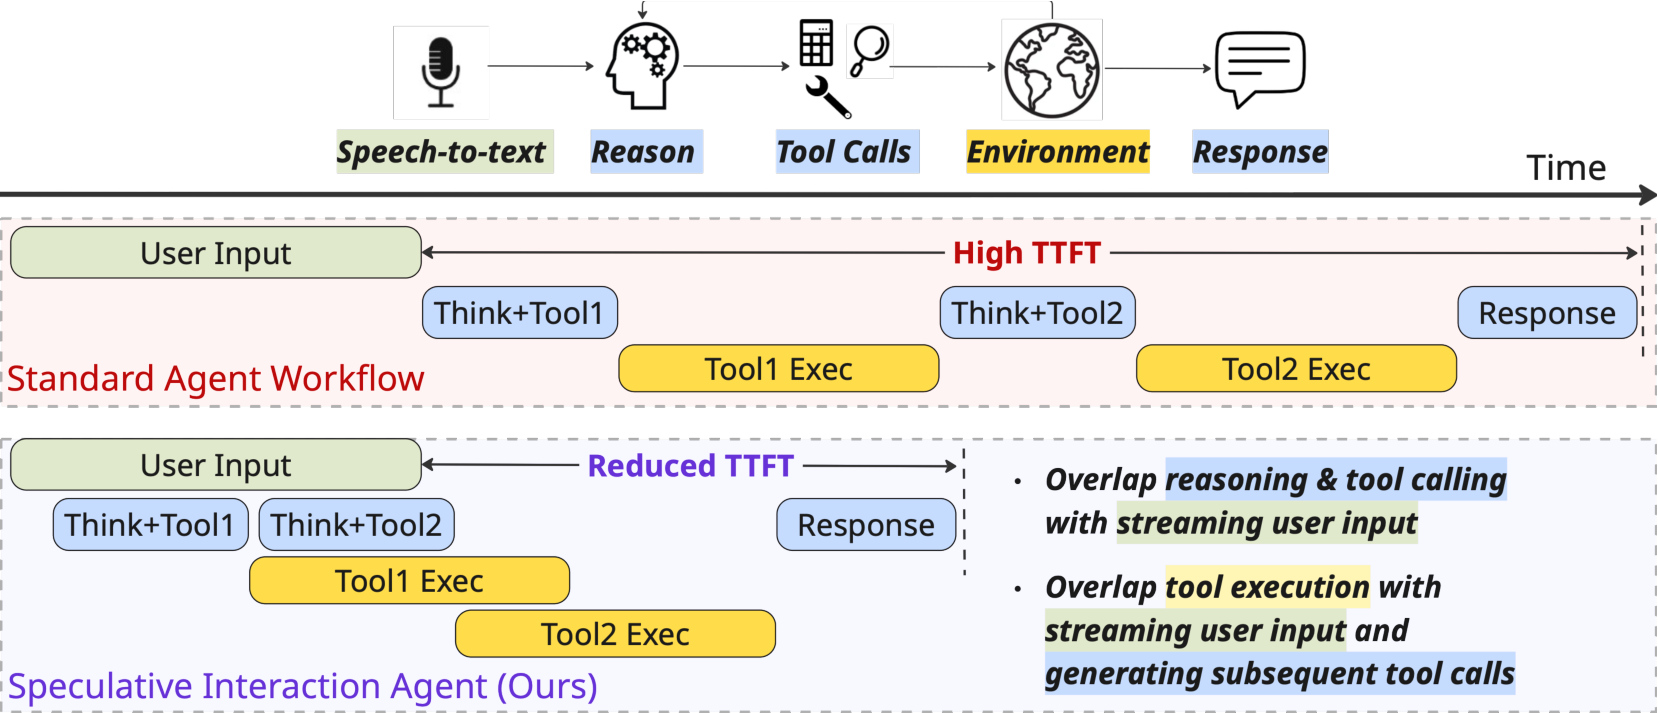
\includegraphics[width=\textwidth]{figures/intro-figure.pdf}
  % \vspace{-7mm}
  \caption{
  \textbf{Overview of Speculative Interaction Agent workflow.} A diagram outlining our proposed workflow in comparison to a standard agentic workflow.
  Standard agentic workflows have high time-to-first-token (TTFT) due to having to wait for the full user response before beginning to think and act on it, as well as having to pause to wait on tool execution.
  Our approach reduces latency by i) overlapping reasoning and acting with the streaming user input (making our agent asynchronous with respect to user inputs), and ii) overlapping reasoning and acting with tool execution (thereby making our agent asynchronous with respect to the environment).
  }
  \label{fig:intro-figure}
  \vspace{-3mm}
\end{figure*}

% problem statement
There is an increasing push for applications that use LLMs as agents, where the model thinks and then executes actions to interact with the external environment \citep{yao2022react,patil2024gorilla,schick2023toolformer}.
This enables the LLM to actuate changes in the real world, for example by looking up information in a database or sending a message.
There has also been growing interest in reasoning models which produce chain-of-thought before answering a question \citep{wei2022chain,guo2025deepseek,qwq32b}. 
Having the model generate this step-by-step chain enhances model accuracy.
However, the increased generation length where the model generates its reasoning process introduces additional latency.

% existing work
Additionally, LLM agents are increasingly leveraged in real-time applications such as customer support and personal assistants.
For many real-time applications, users prefer voice as a medium of interaction to textual inputs via keyboard. 
For voice interactions to feel natural, less than 1 second of latency is typically required \citep{miller1968response}. 
However, if we want the LLM to do any complex agentic workflow which requires reasoning and calling tools, this adds several seconds of latency, which is prohibitive for real-time applications.
This latency comes from both long tool latencies as well as time for the model to reason before each action.

% Comparison against prior work
Previous methods have aimed to accelerate tool calling either through parallelizing tool calls \citep{kim2024llm} or by allowing models to reason while waiting on previous tool calls to execute \citep{gim2024asynchronous}.
Additionally, previous voice agent studies have proposed methods to enable the agent to begin execution before receiving the full input \citep{arora2025stream,chiang2025shanks}.
However, there is no unifying work that allows the model to reason and act while waiting on information from both the user and from the environment.
Additionally, existing methods for voice agents which begin processing based on partial user inputs may launch incorrect tool calls, and existing frameworks lack a method to correct these mistakes while preserving model accuracy.

% Our approach and constributions
In our work, we propose \textit{Speculative Interaction Agents}, which enable real-time interaction by decoupling the agent from the user and environment streams and allowing it to reason and act continuously.
We present our approach assuming streaming input text from speech-to-text using voice as a driving application, but our asynchronous approach is generalizable to any agentic application requiring real-time user interaction.
In particular, our work makes the following contributions:

\vspace{-3mm}
\begin{itemize}
\setlength\itemsep{2pt}
    \item We propose \ASYNCIO, where we decouple the agent's thinking and acting from delays with information arriving from the user and environment (see Section \ref{sec:asynchronous-io}). This decoupling allows the model to work continuously while awaiting updates.
    \item To handle cases where the user has not yet provided complete information, we propose \SPECTOOL, which allows for launching tool calls speculatively and later correcting any mistakes, and which also holds up sensitive tools from execution until they receive final confirmation (see Section \ref{sec:spec-tool-calling}).
    \item We present a clock-based training methodology for training agents to reason and act while waiting for information. We describe how we synthesize trajectories for training models using SFT (see Section \ref{sec:training}).
    \item We also present an inference-time framework which contains a core event-driven agent loop to manage information being received asynchronously from the user and environment, as well as a decoupled task execution module to manage in-flight tool calls (see Section \ref{sec:inference-framework}).
    With our framework, we observe 1.3-1.7$\times$ speedups for cloud real-time APIs and 1.6-2.2$\times$ speedups for edge-scale finetuned models, demonstrating how our approach enables real-time agentic interaction even with agents that have to perform complex multi-turn workflows.
\end{itemize}